Figure \ref{fig:char_fsm_vs_FGI} depicts a comparison of FSM's alignment
process against that of an ICP variant, namely FastGICP, for measurement noise
with $\sigma_R = 0.03$ m. The top figure shows the initial configuration
between two scans captured from poses differing by $\bm{T} = (0.35 \text{m},
0.1 \text{m}, -60 \text{deg})$. While FastGICP progressively reduces the
orientation error, FSM nearly eliminates it in one step. From there it provides
finer approximations of the true orientation by increasing its angular sampling
degree, which in turn allow it to eliminate the positional errors further. The
CAER metric succeeds in navigating the error space better than FastGICP's
internal error metric, especially at such high orientational and positional
displacements. This fact makes FSM suitable in conditions of higher robot
velocities (here up to $4.2$ m/s and $720$ deg/s). FSM converges with an error
of $(0.0098 \text{m}, 0.08 \text{deg})$ in half as many iterations as FastGICP,
whose final error is $(0.61 \text{m}, 9.94 \text{deg})$.

\begin{figure}
    \vspace{0.2cm}
    
\definecolor{pp}{RGB}{0,115,189}
\definecolor{cc}{RGB}{217,84,26}
\definecolor{oo}{RGB}{255,0,255}

% GNUPLOT: LaTeX picture with Postscript
\begingroup
  \makeatletter
  \providecommand\color[2][]{%
    \GenericError{(gnuplot) \space\space\space\@spaces}{%
      Package color not loaded in conjunction with
      terminal option `colourtext'%
    }{See the gnuplot documentation for explanation.%
    }{Either use 'blacktext' in gnuplot or load the package
      color.sty in LaTeX.}%
    \renewcommand\color[2][]{}%
  }%
  \providecommand\includegraphics[2][]{%
    \GenericError{(gnuplot) \space\space\space\@spaces}{%
      Package graphicx or graphics not loaded%
    }{See the gnuplot documentation for explanation.%
    }{The gnuplot epslatex terminal needs graphicx.sty or graphics.sty.}%
    \renewcommand\includegraphics[2][]{}%
  }%
  \providecommand\rotatebox[2]{#2}%
  \@ifundefined{ifGPcolor}{%
    \newif\ifGPcolor
    \GPcolorfalse
  }{}%
  \@ifundefined{ifGPblacktext}{%
    \newif\ifGPblacktext
    \GPblacktexttrue
  }{}%
  % define a \g@addto@macro without @ in the name:
  \let\gplgaddtomacro\g@addto@macro
  % define empty templates for all commands taking text:
  \gdef\gplbacktext{}%
  \gdef\gplfronttext{}%
  \makeatother
  \ifGPblacktext
    % no textcolor at all
    \def\colorrgb#1{}%
    \def\colorgray#1{}%
  \else
    % gray or color?
    \ifGPcolor
      \def\colorrgb#1{\color[rgb]{#1}}%
      \def\colorgray#1{\color[gray]{#1}}%
      \expandafter\def\csname LTw\endcsname{\color{white}}%
      \expandafter\def\csname LTb\endcsname{\color{black}}%
      \expandafter\def\csname LTa\endcsname{\color{black}}%
      \expandafter\def\csname LT0\endcsname{\color[rgb]{1,0,0}}%
      \expandafter\def\csname LT1\endcsname{\color[rgb]{0,1,0}}%
      \expandafter\def\csname LT2\endcsname{\color[rgb]{0,0,1}}%
      \expandafter\def\csname LT3\endcsname{\color[rgb]{1,0,1}}%
      \expandafter\def\csname LT4\endcsname{\color[rgb]{0,1,1}}%
      \expandafter\def\csname LT5\endcsname{\color[rgb]{1,1,0}}%
      \expandafter\def\csname LT6\endcsname{\color[rgb]{0,0,0}}%
      \expandafter\def\csname LT7\endcsname{\color[rgb]{1,0.3,0}}%
      \expandafter\def\csname LT8\endcsname{\color[rgb]{0.5,0.5,0.5}}%
    \else
      % gray
      \def\colorrgb#1{\color{black}}%
      \def\colorgray#1{\color[gray]{#1}}%
      \expandafter\def\csname LTw\endcsname{\color{white}}%
      \expandafter\def\csname LTb\endcsname{\color{black}}%
      \expandafter\def\csname LTa\endcsname{\color{black}}%
      \expandafter\def\csname LT0\endcsname{\color{black}}%
      \expandafter\def\csname LT1\endcsname{\color{black}}%
      \expandafter\def\csname LT2\endcsname{\color{black}}%
      \expandafter\def\csname LT3\endcsname{\color{black}}%
      \expandafter\def\csname LT4\endcsname{\color{black}}%
      \expandafter\def\csname LT5\endcsname{\color{black}}%
      \expandafter\def\csname LT6\endcsname{\color{black}}%
      \expandafter\def\csname LT7\endcsname{\color{black}}%
      \expandafter\def\csname LT8\endcsname{\color{black}}%
    \fi
  \fi
    \setlength{\unitlength}{0.0500bp}%
    \ifx\gptboxheight\undefined%
      \newlength{\gptboxheight}%
      \newlength{\gptboxwidth}%
      \newsavebox{\gptboxtext}%
    \fi%
    \setlength{\fboxrule}{0.5pt}%
    \setlength{\fboxsep}{1pt}%
\begin{picture}(5000.00,6000.00)%
    \gplgaddtomacro\gplbacktext{%
    }%
    \gplgaddtomacro\gplfronttext{%
      \colorrgb{0.00,0.00,0.00}%
      \put(2499,5999){\makebox(0,0){\strut{}\small Initial configuration}}%
    }%
    \gplgaddtomacro\gplbacktext{%
    }%
    \gplgaddtomacro\gplfronttext{%
      \colorrgb{0.00,0.00,0.00}%
      \put(1149,4499){\makebox(0,0){\strut{}\small FastGICP alignment progress}}%
    }%
    \gplgaddtomacro\gplbacktext{%
    }%
    \gplgaddtomacro\gplfronttext{%
      \colorrgb{0.00,0.00,0.00}%
      \put(3849,4499){\makebox(0,0){\strut{}\small FSM alignment progress}}%
    }%
    \gplgaddtomacro\gplbacktext{%
      \colorrgb{0.00,0.45,0.74}%
      \put(368,1800){\makebox(0,0)[r]{\strut{}\scriptsize $0.0$}}%
      \colorrgb{0.00,0.45,0.74}%
      \put(368,1907){\makebox(0,0)[r]{\strut{}\scriptsize $0.2$}}%
      \colorrgb{0.00,0.45,0.74}%
      \put(368,2014){\makebox(0,0)[r]{\strut{}\scriptsize $0.4$}}%
      \colorrgb{0.00,0.45,0.74}%
      \put(368,2121){\makebox(0,0)[r]{\strut{}\scriptsize $0.6$}}%
      \colorrgb{0.00,0.45,0.74}%
      \put(368,2228){\makebox(0,0)[r]{\strut{}\scriptsize $0.8$}}%
      \colorrgb{0.00,0.45,0.74}%
      \put(368,2335){\makebox(0,0)[r]{\strut{}\scriptsize $1.0$}}%
      \colorrgb{0.00,0.45,0.74}%
      \put(368,2442){\makebox(0,0)[r]{\strut{}\scriptsize $1.2$}}%
      \colorrgb{0.00,0.45,0.74}%
      \put(368,2549){\makebox(0,0)[r]{\strut{}\scriptsize $1.4$}}%

      \put(700, 2870){\makebox(0,0){\strut{}{\color{pp}{\rule[0.6mm]{0.5cm}{0.5mm}}} \footnotesize Pos. error [m]}}
      \put(2320,2870){\makebox(0,0){\strut{}{\color{oo}{\rule[0.6mm]{0.5cm}{0.5mm}}} \footnotesize Orient. error [deg]}}
      \put(4120,2870){\makebox(0,0){\strut{}{\color{cc}{\rule[0.6mm]{0.5cm}{0.5mm}}} \footnotesize Internal error metric}}
    }%
    \gplgaddtomacro\gplfronttext{%
    }%
    \gplgaddtomacro\gplbacktext{%
      \colorrgb{0.15,0.15,0.15}%
      \put(400,1680){\makebox(0,0){\strut{}\scriptsize $0$}}%
      \colorrgb{0.15,0.15,0.15}%
      \put(680,1680){\makebox(0,0){\strut{}\scriptsize $10$}}%
      \colorrgb{0.15,0.15,0.15}%
      \put(961,1680){\makebox(0,0){\strut{}\scriptsize $20$}}%
      \colorrgb{0.85,0.33,0.10}%
      \put(1121,1800){\makebox(0,0)[l]{\strut{}}}%
      \colorrgb{0.85,0.33,0.10}%
      \put(1121,1950){\makebox(0,0)[l]{\strut{}}}%
      \colorrgb{0.85,0.33,0.10}%
      \put(1121,2100){\makebox(0,0)[l]{\strut{}}}%
      \colorrgb{0.85,0.33,0.10}%
      \put(1121,2249){\makebox(0,0)[l]{\strut{}}}%
      \colorrgb{0.85,0.33,0.10}%
      \put(1121,2399){\makebox(0,0)[l]{\strut{}}}%
      \colorrgb{0.85,0.33,0.10}%
      \put(1121,2549){\makebox(0,0)[l]{\strut{}}}%
    }%
    \gplgaddtomacro\gplfronttext{%
    }%
    \gplgaddtomacro\gplbacktext{%
      \colorrgb{0.00,0.45,0.74}%
      \put(1368,1800){\makebox(0,0)[r]{\strut{}\scriptsize $0$}}%
      \colorrgb{0.00,0.45,0.74}%
      \put(1368,1931){\makebox(0,0)[r]{\strut{}\scriptsize $10$}}%
      \colorrgb{0.00,0.45,0.74}%
      \put(1368,2061){\makebox(0,0)[r]{\strut{}\scriptsize $20$}}%
      \colorrgb{0.00,0.45,0.74}%
      \put(1368,2192){\makebox(0,0)[r]{\strut{}\scriptsize $30$}}%
      \colorrgb{0.00,0.45,0.74}%
      \put(1368,2323){\makebox(0,0)[r]{\strut{}\scriptsize $40$}}%
      \colorrgb{0.00,0.45,0.74}%
      \put(1368,2454){\makebox(0,0)[r]{\strut{}\scriptsize $50$}}%
    }%
    \gplgaddtomacro\gplfronttext{%
    }%
    \gplgaddtomacro\gplbacktext{%
      \colorrgb{0.15,0.15,0.15}%
      \put(1400,1680){\makebox(0,0){\strut{}\scriptsize $0$}}%
      \colorrgb{0.15,0.15,0.15}%
      \put(1680,1680){\makebox(0,0){\strut{}\scriptsize $10$}}%
      \colorrgb{0.15,0.15,0.15}%
      \put(1961,1680){\makebox(0,0){\strut{}\scriptsize $20$}}%
      \colorrgb{0.85,0.33,0.10}%
      \put(2021,1800){\makebox(0,0)[l]{\strut{}\scriptsize $0$}}%
      \colorrgb{0.85,0.33,0.10}%
      \put(2021,1950){\makebox(0,0)[l]{\strut{}\scriptsize $100$}}%
      \colorrgb{0.85,0.33,0.10}%
      \put(2021,2100){\makebox(0,0)[l]{\strut{}\scriptsize $200$}}%
      \colorrgb{0.85,0.33,0.10}%
      \put(2021,2249){\makebox(0,0)[l]{\strut{}\scriptsize $300$}}%
      \colorrgb{0.85,0.33,0.10}%
      \put(2021,2399){\makebox(0,0)[l]{\strut{}\scriptsize $400$}}%
      \colorrgb{0.85,0.33,0.10}%
      \put(2021,2549){\makebox(0,0)[l]{\strut{}\scriptsize $500$}}%
    }%
    \gplgaddtomacro\gplfronttext{%
    }%
    \gplgaddtomacro\gplbacktext{%
      \colorrgb{0.00,0.45,0.74}%
      \put(2968,1800){\makebox(0,0)[r]{\strut{}\scriptsize $0.0$}}%
      \colorrgb{0.00,0.45,0.74}%
      \put(2968,1987){\makebox(0,0)[r]{\strut{}\scriptsize $0.1$}}%
      \colorrgb{0.00,0.45,0.74}%
      \put(2968,2175){\makebox(0,0)[r]{\strut{}\scriptsize $0.2$}}%
      \colorrgb{0.00,0.45,0.74}%
      \put(2968,2362){\makebox(0,0)[r]{\strut{}\scriptsize $0.3$}}%
      \colorrgb{0.00,0.45,0.74}%
      \put(2968,2549){\makebox(0,0)[r]{\strut{}\scriptsize $0.4$}}%
    }%
    \gplgaddtomacro\gplfronttext{%
    }%
    \gplgaddtomacro\gplbacktext{%
      \colorrgb{0.15,0.15,0.15}%
      \put(3131,1680){\makebox(0,0){\strut{}\scriptsize $2$}}%
      \colorrgb{0.15,0.15,0.15}%
      \put(3262,1680){\makebox(0,0){\strut{}\scriptsize $4$}}%
      \colorrgb{0.15,0.15,0.15}%
      \put(3393,1680){\makebox(0,0){\strut{}\scriptsize $6$}}%
      \colorrgb{0.15,0.15,0.15}%
      \put(3524,1680){\makebox(0,0){\strut{}\scriptsize $8$}}%
      \colorrgb{0.85,0.33,0.10}%
      \put(3721,1800){\makebox(0,0)[l]{\strut{}}}%
      \colorrgb{0.85,0.33,0.10}%
      \put(3721,1987){\makebox(0,0)[l]{\strut{}}}%
      \colorrgb{0.85,0.33,0.10}%
      \put(3721,2175){\makebox(0,0)[l]{\strut{}}}%
      \colorrgb{0.85,0.33,0.10}%
      \put(3721,2362){\makebox(0,0)[l]{\strut{}}}%
      \colorrgb{0.85,0.33,0.10}%
      \put(3721,2549){\makebox(0,0)[l]{\strut{}}}%
    }%
    \gplgaddtomacro\gplfronttext{%
    }%
    \gplgaddtomacro\gplbacktext{%
      \colorrgb{0.00,0.45,0.74}%
      \put(3968,1800){\makebox(0,0)[r]{\strut{}\scriptsize $0$}}%
      \colorrgb{0.00,0.45,0.74}%
      \put(3968,1931){\makebox(0,0)[r]{\strut{}\scriptsize $10$}}%
      \colorrgb{0.00,0.45,0.74}%
      \put(3968,2061){\makebox(0,0)[r]{\strut{}\scriptsize $20$}}%
      \colorrgb{0.00,0.45,0.74}%
      \put(3968,2192){\makebox(0,0)[r]{\strut{}\scriptsize $30$}}%
      \colorrgb{0.00,0.45,0.74}%
      \put(3968,2323){\makebox(0,0)[r]{\strut{}\scriptsize $40$}}%
      \colorrgb{0.00,0.45,0.74}%
      \put(3968,2454){\makebox(0,0)[r]{\strut{}\scriptsize $50$}}%
    }%
    \gplgaddtomacro\gplfronttext{%
    }%
    \gplgaddtomacro\gplbacktext{%
      \colorrgb{0.15,0.15,0.15}%
      \put(4131,1680){\makebox(0,0){\strut{}\scriptsize $2$}}%
      \colorrgb{0.15,0.15,0.15}%
      \put(4262,1680){\makebox(0,0){\strut{}\scriptsize $4$}}%
      \colorrgb{0.15,0.15,0.15}%
      \put(4393,1680){\makebox(0,0){\strut{}\scriptsize $6$}}%
      \colorrgb{0.15,0.15,0.15}%
      \put(4524,1680){\makebox(0,0){\strut{}\scriptsize $8$}}%
      \colorrgb{0.85,0.33,0.10}%
      \put(4621,1800){\makebox(0,0)[l]{\strut{}\scriptsize $0$}}%
      \colorrgb{0.85,0.33,0.10}%
      \put(4621,1987){\makebox(0,0)[l]{\strut{}\scriptsize $50$}}%
      \colorrgb{0.85,0.33,0.10}%
      \put(4621,2175){\makebox(0,0)[l]{\strut{}\scriptsize $100$}}%
      \colorrgb{0.85,0.33,0.10}%
      \put(4621,2362){\makebox(0,0)[l]{\strut{}\scriptsize $150$}}%
      \colorrgb{0.85,0.33,0.10}%
      \put(4621,2549){\makebox(0,0)[l]{\strut{}\scriptsize $200$}}%
    }%
    \gplgaddtomacro\gplfronttext{%
    }%
    \gplgaddtomacro\gplbacktext{%
    }%
    \gplgaddtomacro\gplfronttext{%
      \colorrgb{0.00,0.00,0.00}%
      \put(1149,1379){\makebox(0,0){\strut{}\small FastGICP final alignment}}%
    }%
    \gplgaddtomacro\gplbacktext{%
    }%
    \gplgaddtomacro\gplfronttext{%
      \colorrgb{0.00,0.00,0.00}%
      \put(3849,1379){\makebox(0,0){\strut{}\small FSM final alignment}}%
    }%
    \gplbacktext
    \put(0,0){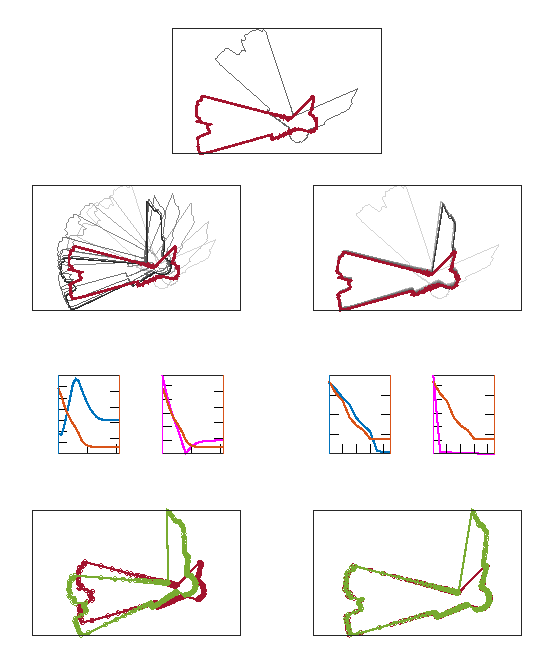
\includegraphics{./figures/characterisation/fsm_vs_fgi}}%
    \gplfronttext
  \end{picture}%
\endgroup

    \caption{\small Comparison of alignment progress of FSM against FastGICP
             for $\sigma_R = 0.03$ m}%
    \label{fig:char_fsm_vs_FGI}%
\end{figure}

Figure \ref{fig:char_max_range_test} shows the behaviour of FSM and an ICP
variant, namely, PLICP, in tests where the sensor's maximum range is limited.
Specifically, it shows their mean orientational and positional errors in ten
tests, for progressively smaller maximum sensor range, within the two
environments depicted in the top row with white colour. The sensor is affected
by noise of $\sigma_R = 0.05$ m. The sensor's first position is marked with a
blue dot. The maximum displacement between sensor poses is set to
$(\overline{\delta}_{xy}, \overline{\delta}_{\theta}) = (0.05 \text{m}, 10 \text{deg})$
and
$(\overline{\delta}_{xy}, \overline{\delta}_{\theta}) = (0.20 \text{m}, 45 \text{deg})$.
Altough one would expect that matching without the use of correspondences would
fare worse than matching with it, FSM exhibits more robust and more accurate
orientational errors than PLICP. In terms of position, FSM's errors are equal to
or lower than those of PLICP.


\begin{figure}\centering
\vspace{-0.2cm}
    \definecolor{rr}{RGB}{227,26,28}
\definecolor{gg}{RGB}{77,176,74}

% GNUPLOT: LaTeX picture with Postscript
\begingroup
  \makeatletter
  \providecommand\color[2][]{%
    \GenericError{(gnuplot) \space\space\space\@spaces}{%
      Package color not loaded in conjunction with
      terminal option `colourtext'%
    }{See the gnuplot documentation for explanation.%
    }{Either use 'blacktext' in gnuplot or load the package
      color.sty in LaTeX.}%
    \renewcommand\color[2][]{}%
  }%
  \providecommand\includegraphics[2][]{%
    \GenericError{(gnuplot) \space\space\space\@spaces}{%
      Package graphicx or graphics not loaded%
    }{See the gnuplot documentation for explanation.%
    }{The gnuplot epslatex terminal needs graphicx.sty or graphics.sty.}%
    \renewcommand\includegraphics[2][]{}%
  }%
  \providecommand\rotatebox[2]{#2}%
  \@ifundefined{ifGPcolor}{%
    \newif\ifGPcolor
    \GPcolorfalse
  }{}%
  \@ifundefined{ifGPblacktext}{%
    \newif\ifGPblacktext
    \GPblacktexttrue
  }{}%
  % define a \g@addto@macro without @ in the name:
  \let\gplgaddtomacro\g@addto@macro
  % define empty templates for all commands taking text:
  \gdef\gplbacktext{}%
  \gdef\gplfronttext{}%
  \makeatother
  \ifGPblacktext
    % no textcolor at all
    \def\colorrgb#1{}%
    \def\colorgray#1{}%
  \else
    % gray or color?
    \ifGPcolor
      \def\colorrgb#1{\color[rgb]{#1}}%
      \def\colorgray#1{\color[gray]{#1}}%
      \expandafter\def\csname LTw\endcsname{\color{white}}%
      \expandafter\def\csname LTb\endcsname{\color{black}}%
      \expandafter\def\csname LTa\endcsname{\color{black}}%
      \expandafter\def\csname LT0\endcsname{\color[rgb]{1,0,0}}%
      \expandafter\def\csname LT1\endcsname{\color[rgb]{0,1,0}}%
      \expandafter\def\csname LT2\endcsname{\color[rgb]{0,0,1}}%
      \expandafter\def\csname LT3\endcsname{\color[rgb]{1,0,1}}%
      \expandafter\def\csname LT4\endcsname{\color[rgb]{0,1,1}}%
      \expandafter\def\csname LT5\endcsname{\color[rgb]{1,1,0}}%
      \expandafter\def\csname LT6\endcsname{\color[rgb]{0,0,0}}%
      \expandafter\def\csname LT7\endcsname{\color[rgb]{1,0.3,0}}%
      \expandafter\def\csname LT8\endcsname{\color[rgb]{0.5,0.5,0.5}}%
    \else
      % gray
      \def\colorrgb#1{\color{black}}%
      \def\colorgray#1{\color[gray]{#1}}%
      \expandafter\def\csname LTw\endcsname{\color{white}}%
      \expandafter\def\csname LTb\endcsname{\color{black}}%
      \expandafter\def\csname LTa\endcsname{\color{black}}%
      \expandafter\def\csname LT0\endcsname{\color{black}}%
      \expandafter\def\csname LT1\endcsname{\color{black}}%
      \expandafter\def\csname LT2\endcsname{\color{black}}%
      \expandafter\def\csname LT3\endcsname{\color{black}}%
      \expandafter\def\csname LT4\endcsname{\color{black}}%
      \expandafter\def\csname LT5\endcsname{\color{black}}%
      \expandafter\def\csname LT6\endcsname{\color{black}}%
      \expandafter\def\csname LT7\endcsname{\color{black}}%
      \expandafter\def\csname LT8\endcsname{\color{black}}%
    \fi
  \fi
    \setlength{\unitlength}{0.0500bp}%
    \ifx\gptboxheight\undefined%
      \newlength{\gptboxheight}%
      \newlength{\gptboxwidth}%
      \newsavebox{\gptboxtext}%
    \fi%
    \setlength{\fboxrule}{0.5pt}%
    \setlength{\fboxsep}{1pt}%
\begin{picture}(5000.00,6000.00)%
    \gplgaddtomacro\gplbacktext{%
    }%
    \gplgaddtomacro\gplfronttext{%
    }%
    \gplgaddtomacro\gplbacktext{%
    }%
    \gplgaddtomacro\gplfronttext{%
    }%
    \gplgaddtomacro\gplbacktext{%
    }%
    \gplgaddtomacro\gplfronttext{%
      \colorrgb{0.00,0.00,0.00}%
      \put(2587,4390){\makebox(0,0){\strut{}\small Proportion of rays' ranges within maximum sensor range}}%
      \put(2070,3670){\makebox(0,0){\strut{}{\color{rr}{\rule[0.6mm]{0.5cm}{0.5mm}}} \footnotesize CSM}}
      \put(3070,3670){\makebox(0,0){\strut{}{\color{gg}{\rule[0.6mm]{0.5cm}{0.5mm}}} \footnotesize FSM}}
      \put(850,3420){\makebox(0,0){\strut{} \footnotesize Conf$_a$}}
      \put(1890,3420){\makebox(0,0){\strut{} \footnotesize Conf$_b$}}
      \put(3300,3420){\makebox(0,0){\strut{} \footnotesize Conf$_a$}}
      \put(4340,3420){\makebox(0,0){\strut{} \footnotesize Conf$_b$}}
    }%
    \gplgaddtomacro\gplbacktext{%
    }%
    \gplgaddtomacro\gplfronttext{%
      \colorrgb{0.15,0.15,0.15}%
      \put(650,3980){\makebox(0,0){\strut{}\scriptsize $0\%$}}%
      \colorrgb{0.15,0.15,0.15}%
      \put(1425,3980){\makebox(0,0){\strut{}\scriptsize $20\%$}}%
      \colorrgb{0.15,0.15,0.15}%
      \put(2200,3980){\makebox(0,0){\strut{}\scriptsize $40\%$}}%
      \colorrgb{0.15,0.15,0.15}%
      \put(2974,3980){\makebox(0,0){\strut{}\scriptsize $60\%$}}%
      \colorrgb{0.15,0.15,0.15}%
      \put(3749,3980){\makebox(0,0){\strut{}\scriptsize $80\%$}}%
      \colorrgb{0.15,0.15,0.15}%
      \put(4524,3980){\makebox(0,0){\strut{}\scriptsize $100\%$}}%
    }%
    \gplgaddtomacro\gplbacktext{%
      \colorrgb{0.15,0.15,0.15}%
      \put(448,2400){\makebox(0,0)[r]{\strut{}\scriptsize $0$}}%
      \colorrgb{0.15,0.15,0.15}%
      \put(448,2550){\makebox(0,0)[r]{\strut{}\scriptsize $2$}}%
      \colorrgb{0.15,0.15,0.15}%
      \put(448,2700){\makebox(0,0)[r]{\strut{}\scriptsize $4$}}%
      \colorrgb{0.15,0.15,0.15}%
      \put(448,2850){\makebox(0,0)[r]{\strut{}\scriptsize $6$}}%
      \colorrgb{0.15,0.15,0.15}%
      \put(448,2999){\makebox(0,0)[r]{\strut{}\scriptsize $8$}}%
      \colorrgb{0.15,0.15,0.15}%
      \put(448,3149){\makebox(0,0)[r]{\strut{}\scriptsize $10$}}%
      \colorrgb{0.15,0.15,0.15}%
      \put(448,3299){\makebox(0,0)[r]{\strut{}\scriptsize $12$}}%
      \colorrgb{0.15,0.15,0.15}%
      \put(500,2180){\makebox(0,0){\strut{}}}%
      \colorrgb{0.15,0.15,0.15}%
      \put(650,2180){\makebox(0,0){\strut{}}}%
      \colorrgb{0.15,0.15,0.15}%
      \put(800,2180){\makebox(0,0){\strut{}}}%
      \colorrgb{0.15,0.15,0.15}%
      \put(949,2180){\makebox(0,0){\strut{}}}%
      \colorrgb{0.15,0.15,0.15}%
      \put(1099,2180){\makebox(0,0){\strut{}}}%
      \colorrgb{0.15,0.15,0.15}%
      \put(1249,2180){\makebox(0,0){\strut{}}}%
    }%
    \gplgaddtomacro\gplfronttext{%
      \colorrgb{0.15,0.15,0.15}%
      \put(40,2849){\rotatebox{90}{\makebox(0,0){\strut{}$e_{orient}$ [deg]}}}%
    }%
    \gplgaddtomacro\gplbacktext{%
      \colorrgb{0.15,0.15,0.15}%
      \put(1498,2400){\makebox(0,0)[r]{\strut{}\scriptsize $0$}}%
      \colorrgb{0.15,0.15,0.15}%
      \put(1498,2625){\makebox(0,0)[r]{\strut{}\scriptsize $10$}}%
      \colorrgb{0.15,0.15,0.15}%
      \put(1498,2850){\makebox(0,0)[r]{\strut{}\scriptsize $20$}}%
      \colorrgb{0.15,0.15,0.15}%
      \put(1498,3074){\makebox(0,0)[r]{\strut{}\scriptsize $30$}}%
      \colorrgb{0.15,0.15,0.15}%
      \put(1498,3299){\makebox(0,0)[r]{\strut{}\scriptsize $40$}}%
      \colorrgb{0.15,0.15,0.15}%
      \put(1550,2180){\makebox(0,0){\strut{}}}%
      \colorrgb{0.15,0.15,0.15}%
      \put(1700,2180){\makebox(0,0){\strut{}}}%
      \colorrgb{0.15,0.15,0.15}%
      \put(1850,2180){\makebox(0,0){\strut{}}}%
      \colorrgb{0.15,0.15,0.15}%
      \put(1999,2180){\makebox(0,0){\strut{}}}%
      \colorrgb{0.15,0.15,0.15}%
      \put(2149,2180){\makebox(0,0){\strut{}}}%
      \colorrgb{0.15,0.15,0.15}%
      \put(2299,2180){\makebox(0,0){\strut{}}}%
    }%
    \gplgaddtomacro\gplfronttext{%
    }%
    \gplgaddtomacro\gplbacktext{%
      \colorrgb{0.15,0.15,0.15}%
      \put(2898,2400){\makebox(0,0)[r]{\strut{}\scriptsize $0$}}%
      \colorrgb{0.15,0.15,0.15}%
      \put(2898,2580){\makebox(0,0)[r]{\strut{}\scriptsize $2$}}%
      \colorrgb{0.15,0.15,0.15}%
      \put(2898,2760){\makebox(0,0)[r]{\strut{}\scriptsize $4$}}%
      \colorrgb{0.15,0.15,0.15}%
      \put(2898,2939){\makebox(0,0)[r]{\strut{}\scriptsize $6$}}%
      \colorrgb{0.15,0.15,0.15}%
      \put(2898,3119){\makebox(0,0)[r]{\strut{}\scriptsize $8$}}%
      \colorrgb{0.15,0.15,0.15}%
      \put(2898,3299){\makebox(0,0)[r]{\strut{}\scriptsize $10$}}%
      \colorrgb{0.15,0.15,0.15}%
      \put(2950,2180){\makebox(0,0){\strut{}}}%
      \colorrgb{0.15,0.15,0.15}%
      \put(3100,2180){\makebox(0,0){\strut{}}}%
      \colorrgb{0.15,0.15,0.15}%
      \put(3250,2180){\makebox(0,0){\strut{}}}%
      \colorrgb{0.15,0.15,0.15}%
      \put(3399,2180){\makebox(0,0){\strut{}}}%
      \colorrgb{0.15,0.15,0.15}%
      \put(3549,2180){\makebox(0,0){\strut{}}}%
      \colorrgb{0.15,0.15,0.15}%
      \put(3699,2180){\makebox(0,0){\strut{}}}%
    }%
    \gplgaddtomacro\gplfronttext{%
    }%
    \gplgaddtomacro\gplbacktext{%
      \colorrgb{0.15,0.15,0.15}%
      \put(3948,2400){\makebox(0,0)[r]{\strut{}\scriptsize $0$}}%
      \colorrgb{0.15,0.15,0.15}%
      \put(3948,2625){\makebox(0,0)[r]{\strut{}\scriptsize $10$}}%
      \colorrgb{0.15,0.15,0.15}%
      \put(3948,2850){\makebox(0,0)[r]{\strut{}\scriptsize $20$}}%
      \colorrgb{0.15,0.15,0.15}%
      \put(3948,3074){\makebox(0,0)[r]{\strut{}\scriptsize $30$}}%
      \colorrgb{0.15,0.15,0.15}%
      \put(3948,3299){\makebox(0,0)[r]{\strut{}\scriptsize $40$}}%
      \colorrgb{0.15,0.15,0.15}%
      \put(4000,2180){\makebox(0,0){\strut{}}}%
      \colorrgb{0.15,0.15,0.15}%
      \put(4150,2180){\makebox(0,0){\strut{}}}%
      \colorrgb{0.15,0.15,0.15}%
      \put(4300,2180){\makebox(0,0){\strut{}}}%
      \colorrgb{0.15,0.15,0.15}%
      \put(4449,2180){\makebox(0,0){\strut{}}}%
      \colorrgb{0.15,0.15,0.15}%
      \put(4599,2180){\makebox(0,0){\strut{}}}%
      \colorrgb{0.15,0.15,0.15}%
      \put(4749,2180){\makebox(0,0){\strut{}}}%
    }%
    \gplgaddtomacro\gplfronttext{%
    }%
    \gplgaddtomacro\gplbacktext{%
      \colorrgb{0.15,0.15,0.15}%
      \put(448,1260){\makebox(0,0)[r]{\strut{}\scriptsize $0$}}%
      \colorrgb{0.15,0.15,0.15}%
      \put(448,1560){\makebox(0,0)[r]{\strut{}\scriptsize $2$}}%
      \colorrgb{0.15,0.15,0.15}%
      \put(448,1859){\makebox(0,0)[r]{\strut{}\scriptsize $4$}}%
      \colorrgb{0.15,0.15,0.15}%
      \put(448,2159){\makebox(0,0)[r]{\strut{}\scriptsize $6$}}%
      \colorrgb{0.15,0.15,0.15}%
      \put(500,1040){\makebox(0,0){\strut{}}}%
      \colorrgb{0.15,0.15,0.15}%
      \put(650,1040){\makebox(0,0){\strut{}\scriptsize $20$}}%
      \colorrgb{0.15,0.15,0.15}%
      \put(800,1040){\makebox(0,0){\strut{}}}%
      \colorrgb{0.15,0.15,0.15}%
      \put(949,1040){\makebox(0,0){\strut{}\scriptsize $60$}}%
      \colorrgb{0.15,0.15,0.15}%
      \put(1099,1040){\makebox(0,0){\strut{}}}%
      \colorrgb{0.15,0.15,0.15}%
      \put(1249,1040){\makebox(0,0){\strut{}\scriptsize $100$}}%
    }%
    \gplgaddtomacro\gplfronttext{%
      \colorrgb{0.15,0.15,0.15}%
      \put(40,1709){\rotatebox{90}{\makebox(0,0){\strut{}$e_{pos}$ [cm]}}}%
    }%
    \gplgaddtomacro\gplbacktext{%
      \colorrgb{0.15,0.15,0.15}%
      \put(1498,1260){\makebox(0,0)[r]{\strut{}\scriptsize $0$}}%
      \colorrgb{0.15,0.15,0.15}%
      \put(1498,1485){\makebox(0,0)[r]{\strut{}\scriptsize $5$}}%
      \colorrgb{0.15,0.15,0.15}%
      \put(1498,1710){\makebox(0,0)[r]{\strut{}\scriptsize $10$}}%
      \colorrgb{0.15,0.15,0.15}%
      \put(1498,1934){\makebox(0,0)[r]{\strut{}\scriptsize $15$}}%
      \colorrgb{0.15,0.15,0.15}%
      \put(1498,2159){\makebox(0,0)[r]{\strut{}\scriptsize $20$}}%
      \colorrgb{0.15,0.15,0.15}%
      \put(1550,1040){\makebox(0,0){\strut{}}}%
      \colorrgb{0.15,0.15,0.15}%
      \put(1700,1040){\makebox(0,0){\strut{}\scriptsize $20$}}%
      \colorrgb{0.15,0.15,0.15}%
      \put(1850,1040){\makebox(0,0){\strut{}}}%
      \colorrgb{0.15,0.15,0.15}%
      \put(1999,1040){\makebox(0,0){\strut{}\scriptsize $60$}}%
      \colorrgb{0.15,0.15,0.15}%
      \put(2149,1040){\makebox(0,0){\strut{}}}%
      \colorrgb{0.15,0.15,0.15}%
      \put(2299,1040){\makebox(0,0){\strut{}\scriptsize $100$}}%
    }%
    \gplgaddtomacro\gplfronttext{%
    }%
    \gplgaddtomacro\gplbacktext{%
      \colorrgb{0.15,0.15,0.15}%
      \put(2898,1260){\makebox(0,0)[r]{\strut{}\scriptsize $0$}}%
      \colorrgb{0.15,0.15,0.15}%
      \put(2898,1560){\makebox(0,0)[r]{\strut{}\scriptsize $2$}}%
      \colorrgb{0.15,0.15,0.15}%
      \put(2898,1859){\makebox(0,0)[r]{\strut{}\scriptsize $4$}}%
      \colorrgb{0.15,0.15,0.15}%
      \put(2898,2159){\makebox(0,0)[r]{\strut{}\scriptsize $6$}}%
      \colorrgb{0.15,0.15,0.15}%
      \put(2950,1040){\makebox(0,0){\strut{}}}%
      \colorrgb{0.15,0.15,0.15}%
      \put(3100,1040){\makebox(0,0){\strut{}\scriptsize $20$}}%
      \colorrgb{0.15,0.15,0.15}%
      \put(3250,1040){\makebox(0,0){\strut{}}}%
      \colorrgb{0.15,0.15,0.15}%
      \put(3399,1040){\makebox(0,0){\strut{}\scriptsize $60$}}%
      \colorrgb{0.15,0.15,0.15}%
      \put(3549,1040){\makebox(0,0){\strut{}}}%
      \colorrgb{0.15,0.15,0.15}%
      \put(3699,1040){\makebox(0,0){\strut{}\scriptsize $100$}}%
    }%
    \gplgaddtomacro\gplfronttext{%
    }%
    \gplgaddtomacro\gplbacktext{%
      \colorrgb{0.15,0.15,0.15}%
      \put(3948,1260){\makebox(0,0)[r]{\strut{}\scriptsize $0$}}%
      \colorrgb{0.15,0.15,0.15}%
      \put(3948,1485){\makebox(0,0)[r]{\strut{}\scriptsize $5$}}%
      \colorrgb{0.15,0.15,0.15}%
      \put(3948,1710){\makebox(0,0)[r]{\strut{}\scriptsize $10$}}%
      \colorrgb{0.15,0.15,0.15}%
      \put(3948,1934){\makebox(0,0)[r]{\strut{}\scriptsize $15$}}%
      \colorrgb{0.15,0.15,0.15}%
      \put(3948,2159){\makebox(0,0)[r]{\strut{}\scriptsize $20$}}%
      \colorrgb{0.15,0.15,0.15}%
      \put(4000,1040){\makebox(0,0){\strut{}}}%
      \colorrgb{0.15,0.15,0.15}%
      \put(4150,1040){\makebox(0,0){\strut{}\scriptsize $20$}}%
      \colorrgb{0.15,0.15,0.15}%
      \put(4300,1040){\makebox(0,0){\strut{}}}%
      \colorrgb{0.15,0.15,0.15}%
      \put(4449,1040){\makebox(0,0){\strut{}\scriptsize $60$}}%
      \colorrgb{0.15,0.15,0.15}%
      \put(4599,1040){\makebox(0,0){\strut{}}}%
      \colorrgb{0.15,0.15,0.15}%
      \put(4749,1040){\makebox(0,0){\strut{}\scriptsize $100$}}%
    }%
    \gplgaddtomacro\gplfronttext{%
    }%
    \gplbacktext
    \put(0,0){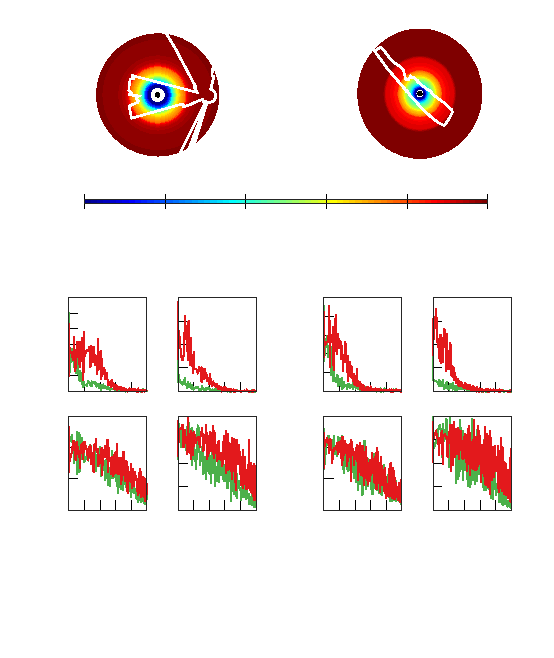
\includegraphics{./figures/characterisation/max_range_test}}%
    \gplfronttext
  \end{picture}%
\endgroup

    \vspace{-1.5cm}
    \caption{\small FSM's performance with respect to receding maximum sensor
             range, compared to that of PLICP. Conf$_a$ is configuration
             $(\overline{\delta}_{xy}, \overline{\delta}_{\theta}) = (0.05 \text{m}, 10 \text{deg})$.
             Conf$_b$ is
             $(\overline{\delta}_{xy}, \overline{\delta}_{\theta}) = (0.20 \text{m}, 45 \text{deg})$
             }%
    \label{fig:char_max_range_test}%
\end{figure}
